%%
%% Copyright 2007, 2008, 2009 Elsevier Ltd
%%
%% This file is part of the 'Elsarticle Bundle'.
%% ---------------------------------------------
%%
%% It may be distributed under the conditions of the LaTeX Project Public
%% License, either version 1.2 of this license or (at your option) any
%% later version.  The latest version of this license is in
%%    http://www.latex-project.org/lppl.txt
%% and version 1.2 or later is part of all distributions of LaTeX
%% version 1999/12/01 or later.
%%
%% The list of all files belonging to the 'Elsarticle Bundle' is
%% given in the file `manifest.txt'.
%%

%% Template article for Elsevier's document class `elsarticle'
%% with numbered style bibliographic references
%% SP 2008/03/01

\documentclass[preprint,12pt, a4paper]{elsarticle}

%% Use the option review to obtain double line spacing
%% \documentclass[authoryear,preprint,review,12pt]{elsarticle}

%% For including figures, graphicx.sty has been loaded in
%% elsarticle.cls. If you prefer to use the old commands
%% please give \usepackage{epsfig}

%% The amssymb package provides various useful mathematical symbols
\usepackage{amssymb}
%% The amsthm package provides extended theorem environments
\usepackage{amsthm}
\usepackage{amsmath}
\usepackage{mathtools}
%% The lineno packages adds line numbers. Start line numbering with
%% \begin{linenumbers}, end it with \end{linenumbers}. Or switch it on
%% for the whole article with \linenumbers.
\usepackage{lineno}

\usepackage{float}

\usepackage{todonotes}
\usepackage{url}

\restylefloat{table}

\newcommand{\eg}{{\emph{e.g.\/}}}
\newcommand{\ie}{{\emph{i.e.\/}}}
\newcommand{\ket}[1]{\ensuremath{|#1\rangle}}
\newcommand{\bra}[1]{\ensuremath{\langle#1|}}
\newcommand{\ketbra}[2]{\ensuremath{\ket{#1}\bra{#2}}}
\newcommand{\proj}[1]{\ensuremath{\ketbra{#1}{#1}}}
\newcommand{\braket}[2]{\ensuremath{\langle{#1}|{#2}\rangle}}
\newcommand{\floor}[1]{\ensuremath{\lfloor #1 \rfloor}}
\newcommand{\complexity}[1]{\ensuremath{\mathbf{#1}}}
\newcommand{\new}[1]{ \textcolor{red}{#1} }
\newcommand{\1}{{\rm 1\hspace{-0.9mm}l}}
\newcommand{\Id}{{\rm 1\hspace{-0.9mm}l}}
\newcommand{\connected}{\sim}
\newcommand{\SPAN}{\mathrm{span}}
\newcommand{\Lrm}{\ensuremath{\mathrm{L}}}
\newcommand{\Urm}{\ensuremath{\mathrm{U}}}
\newcommand{\ee}{\ensuremath{\mathrm{e}}}
\newcommand{\dd}{\ensuremath{\mathrm{d}}}
\newcommand{\ii}{\ensuremath{\mathrm{i}}}
\newcommand{\EE}{\mathcal{E}}
\newcommand{\XX}{\mathcal{X}}
\newcommand{\MM}{\mathcal{M}}
\newcommand{\NN}{\mathcal{N}}
\newcommand{\DD}{\mathcal{D}}
\newcommand{\TT}{\mathcal{T}}
\newcommand{\PP}{\mathcal{P}}
\newcommand{\QQ}{\mathcal{Q}}
\renewcommand{\SS}{\mathcal{S}}
\newcommand{\UU}{\mathcal{U}}
\newcommand{\HH}{\mathcal{H}}
\newcommand{\DU}{\mathcal{DU}}
\newcommand{\NOT}{\sigma_x}
\newcommand{\idop}[1][\XX]{\ensuremath{\1_{#1}}}
\newcommand{\diaguni}{\ensuremath{\mathcal{DU}}}
\newcommand{\diag}{\mathrm{diag}}
\newcommand{\tr}{\mathrm{tr}}
%\DeclareMathOperator{\diag}{diag}
%\DeclareMathOperator{\diag}{diag}
\journal{SoftwareX}


\usepackage{amsmath}
\newtheorem{theorem}{Theorem}
\newtheorem{proposition}{Proposition}
\newtheorem{remark}{Remark}
\newtheorem{scheme}{Scheme}
\newtheorem{lemma}{Lemma}

\begin{document}



\subsubsection{Motivation}

Suppose we have access to a device performing one of the predefined von Neumann
measurements\footnote{In PyQBench, we restrict ourselves to discriminating von Neumann measurements.
This is because, unlike other measurement types, they can be implemented on actual hardware.
},  $\PP$ or $\QQ$. While the $\PP$ and $\QQ$ are known, it is not known which of them is
performed when the device executes. Based on the measurement outcome, you have to guess which
measurement was performed (but you can perform arbitrary unitary operations before and after the
measurement). What is the highest probability of making a correct guess? And what do you have to do
to achieve it? And, most importantly, why would we want to do this?

Suppose that you know a strategy that, for an ideal device, would yield a probability
$p_{\text{succ}}$ of successfully discriminating between two measurements. Will the probability be
the same on an actual physical device? For current, Noisy Intermediate Scale Quantum devices
(NISQs), the answer is: certainly not. However, the error rate that you make when guessing can be
used as a benchmarking metric. PyQBench helps you in organizing such discrimination experiments for
a single qubit system\footnote{As we will soon see, the optimal discrimination strategy requires
the usage of an additional auxiliary qubit.}, executing them on real hardware or simulators, and
computing discrimination probabilities based on the measured bitstrings.

\subsubsection{Notation and some preliminaries}


Recall that a general quantum
measurement, that is a positive operator valued measure (POVM) $\PP$ is a
collection of positive semidefinite operators $\{E_1, \ldots, E_m \}$ called
\emph{effects}, which sum up to identity, \ie $ \, \, \sum_{i=1}^m E_i = \1$.
In PyQBench, we are interested only in von Neumann measurements, i.e. measurements
for which all the effects are rank-one projectors. Every such measurement can be
parameterized by a unitary matrix $U$ which the effects $\{\proj{u_0}, \ldots, \proj{u_{d-1}}\}$,
are created by taking $\ket{u_i}$ as  $i+1$-th column of the unitary matrix $U$.
We will denote von Neumann measurements described by the matrix $U$ by $\PP_{U}$.

Typically, NISQ devices can only perform measurements in computational $Z$-basis.
To perform an arbitrary von Neumann measurement $\PP_{U}$, one has to first apply $U^\dagger$
to the measured system and then follow with $Z$-basis measurement. Hence, the following two
circuits are equivalent.

\begin{figure}[h!]
	\centering
	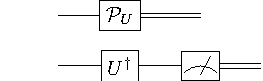
\includegraphics[scale=1.7]{pics/vonneuman}
	\caption{Decomposition of von Neumann measurement}
	\label{fig:vonnneuman}
\end{figure}

Note that the decomposition above is basically a change of basis in which the measurement
is performed.

\subsubsection{Discrimination scheme}

Without loss of generality, we consider discrimination between a measurement in the computational
Z-basis ($\PP_\Id$), and an alternative measurement performed in the basis $U$
($\PP_U$)\footnote{Explaining why we can consider only Z-basis and alternative measurement is beyond
the scope of this technical documentation. See \cite{puchala2018strategies} if you are interested in
the explanation.}. In PyQBench, we operate only on two-level systems, but the discrimination scheme,
described in detail in \cite{puchala2018strategies}, makes no assumptions about the dimensionality.

In general, the discrimination scheme, presented in Fig.\ref{fig:theoretical_scheme}, requires a
second system of the same dimensionality as the measured one. First, the joint system is prepared in
some state $\ket{\psi_0}$. Then, the unknown measurement is performed on the first part of the
system. Based on its outcome $i$, another measurement $\mathcal{P}_{V_i}$ is performed to obtain an
outcome $j$. Finally, if $j=0$ we guess that the performed measurement is $\mathcal{P}_U$, otherwise
we guess that it was $\mathcal{P}_\Id$.

\begin{figure}[h!]
	\centering
	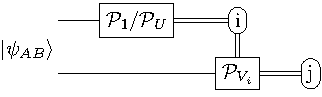
\includegraphics[scale=1.7]{pics/theoretical_scheme}
	\caption{Theoretical  scheme of discrimination  between von Neumann measurements $\PP_{U}$ and $\PP_\Id$. }
	\label{fig:theoretical_scheme}
\end{figure}

\subsubsection{Limitations of NISQ devices and practical discrimination schemes}

Current NISQ devices are unable to perform conditional measurements, which is the biggest
obstacle to implementing our scheme on real hardware. Luckily, we can overcome it by
cleverly adjusting our scheme so that it only uses components available on current devices.
We have two possible choices here: using a postselection or a direct sum
$V_0^\dagger\oplus V_1^\dagger$.

\begin{scheme}(By using postselection)

The first idea is very simple. Instead of performing a conditional measurement, for each
measurement $\PP_U, \PP_\Id$ to be discriminated and each choice of $k \in \{0, 1\}$ we run circuit presented in Fig. \ref{fig:postselection}.

\begin{figure}[h!]
	\centering
	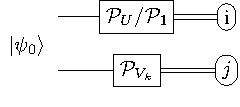
\includegraphics[scale=1.7]{pics/postselection_no_channels}

	\caption{
		Postselection scheme of discrimination between von Neumann measurements $\PP_{U}$ and $\PP_\Id$.
	}\label{fig:postselection}
\end{figure}




\begin{enumerate}
	\item We prepare the discriminator $\ket{\psi_{0}}$ on bipartite
	system.
	%\item We perform one of two quantum channels, either $\Phi_{\Id}$ or
	%$\Phi_{U^\dagger}$,  on  the first part of the input state  $\ket{\psi_{0}}$, that means $\left(\Phi \otimes \Id\right)(\proj{\psi_0})$.
	\item We apply one of unitary,   either $U^\dagger$ or
	$\Id$, on the first system.
	%\item Based on Holevo--Helstrom theorem, we perform a conditional binary measurement $\PP_{V_j}$, and hence, we implement the direct sum of quantum channels $\Phi_{V_0^\dagger} \oplus \Phi_{V_1^\dagger}$. Observe that   $\Phi_{V_0^\dagger} \oplus \Phi_{V_1^\dagger} = \proj{0} \otimes \Phi_{V_0^\dagger}  + \proj{1} \otimes \Phi_{V_1^\dagger}.  $
	\item We apply one of unitary  $V_0^\dagger $ or $V_1^\dagger$ on the second system.
	\item We measure both systems in computational basis $\Delta$.
	\item We make a decision based on the received label $i$  and $j$. The details about the method of probability calculation is described below.
\end{enumerate} 


But now our experiment does not match the previously described scheme, right?
Yes, unless we discard all the outcomes for which $i\ne k$ (hence the name \emph{postselection},
we are selecting valid outcomes after the experiment is performed).

% \begin{scheme}(Postselection)

% %\begin{figure}[h!]
% %	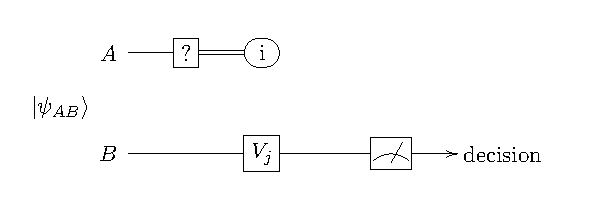
\includegraphics[scale=1.5]{onequbit.pdf}
% %	\caption{A schematic representation of the setup for distinguishing
% %		measurements using postselection.}
% %	\label{postselection}
% %\end{figure}

% \begin{enumerate}
% \item We prepare  the discriminator $\ket{\psi_{0}}$ on bipartite system.
% \item We perform one of two quantum channels, either $\Phi_{\Id}$ or
% $\Phi_{U^\dagger}$,  on  the first part of the input state  $\ket{\psi_{0}}$, that means $\left( \Phi \otimes \Id\right)(\proj{\psi_0})$.
% \item We measure the first part of the input state  $\ket{\psi_{0}}$ and
% receive an output label $i$.
% \item
% Based on Holevo--Helstrom theorem, we perform a conditional binary
% measurement	$\PP_{V_j}$ and hence, we implement the quantum channel $\Phi_{V_j^\dagger}$ on the second part.
% \item To calculate the probability of correct discrimination, we include just those cases for which $i = j$.
% \item We measure the second part of the input state  $\ket{\psi_{0}}$ and make a
% decision based on received label $j$. If $i=j=0$, then we decide that
% $\PP_U$ occurs.  If $i=j=1$, we decide that
% $\PP_{\Id}$ occurs.
% \end{enumerate}

More precisely, our experiments can be grouped into classes identified by tuples of the form
$(\mathcal{Q}, k, i, j)$, where $\mathcal{Q} \in \{\PP_U, \PP_\Id\}$ denotes the chosen measurement.
We discard all the experiments for which $k \ne i$. Hence, the total number of valid experiments is

\begin{equation}
	N_\text{total} = \#\{(\QQ, k, i, j): k = i \}. 
\end{equation}

We now need to count the experiments (among the valid ones) resulting in successful discrimination.
If we have chosen $\PP_U$, then we guess correctly iff $j=0$. Similarly, for
$P_\Id$, we guess correctly iff $j=1$. If we define
\begin{eqnarray}
	N_{\PP_U} &= \#\{(\mathcal{Q}, k, i, j): \mathcal{Q} = \PP_U, k = i, j = 0\}, \\
	N_{\PP_\Id} &= \#\{(\mathcal{Q}, k, i, j): \mathcal{Q} = \PP_\Id, k = i, j = 1\},
\end{eqnarray}
then the empirical success probability can be computed as

\begin{equation}
p_{\text{succ}}(\PP_{U}, \PP_{\Id}) = \frac{N_{\PP_U} + N_{\PP_\Id}}{N_{\text{total}}}.
\end{equation}

\end{scheme}

\begin{scheme}(By using direct sum)



\begin{enumerate}
\item We prepare the discriminator $\ket{\psi_{0}}$ on bipartite
system.
%\item We perform one of two quantum channels, either $\Phi_{\Id}$ or
%$\Phi_{U^\dagger}$,  on  the first part of the input state  $\ket{\psi_{0}}$, that means $\left(\Phi \otimes \Id\right)(\proj{\psi_0})$.
\item We apply one of unitary,   either $U^\dagger$ or
$\Id$, on the first system.
%\item Based on Holevo--Helstrom theorem, we perform a conditional binary measurement $\PP_{V_j}$, and hence, we implement the direct sum of quantum channels $\Phi_{V_0^\dagger} \oplus \Phi_{V_1^\dagger}$. Observe that   $\Phi_{V_0^\dagger} \oplus \Phi_{V_1^\dagger} = \proj{0} \otimes \Phi_{V_0^\dagger}  + \proj{1} \otimes \Phi_{V_1^\dagger}.  $
\item We apply direct sum $V_0^\dagger \oplus V_1^\dagger$ on the whole systems.
\item We measure both systems in computational basis $\Delta$.
\item We make a decision based on the received label $j$ on the second system. If $j=0$, then we
decide that $\PP_U$ occurs. Otherwise, we decide that $\PP_{\Id}$ occurs.
\end{enumerate}

The schematic representation of this setup is depicted in
Fig.~\ref{fig:controlled}.
\begin{figure}[h!]
	\centering
	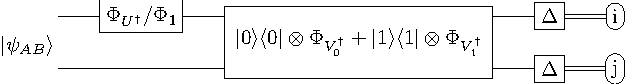
\includegraphics[scale=1.5]{pics/controlled_unitary}

	\caption{ A schematic representation of the setup for distinguishing
		measurements using controlled unitary gate.
	}\label{fig:controlled}
\end{figure}

In this scheme, the experiment can be characterized by a pair $(\mathcal{Q}, i,j)$, where $\mathcal{Q} = \{ \PP_{U}, \PP_{\Id} \}$. The number of successful trials for $U$ and $\Id$, respectively, can be written  as
\begin{eqnarray}
N_{\PP_U} &= \#\{(\mathcal{Q},  i, j): \mathcal{Q} = \PP_U, j = 0\}, \\
N_{\PP_\Id} &= \#\{(\mathcal{Q},  i, j): \mathcal{Q} = \PP_\Id, j = 1\}.
\end{eqnarray}
Then, the probability of correct discrimination between $\PP_{U} $ and $\PP_\Id$ is given by
\begin{equation}
p_{\text{succ}} = \frac{N_{\PP_{U}} + N_{\PP_{\Id}}}{N_{\text{total}}},
\end{equation}
where $N_{\text{total}}$ is the number of trials.
\end{scheme}




\subsubsection{Optimal discrimination scheme}


The celebrated result by Helstrom~\cite{helstrom1976quantum} gives the optimal  probability of correct discrimination between two quantum measurements, $\PP$  and $\mathcal{Q}$,
in terms of their distance with the use of the diamond norm
\begin{equation}
p_{\text{succ}}(\PP, \mathcal{Q}) =  \frac12 + \frac14 \| \PP - \mathcal{Q} \|_\diamond, 
\end{equation}
where 
\begin{equation}
\|\PP\|_\diamond = \max_{\| \ket{\psi}\|_1=1} \| \left(\PP \otimes \1\right) (\proj{\psi}) \|_1.
\end{equation}
The quantum state $\ket{\psi}$ which maximizes the diamond norm is called as discriminator.
Furthermore,  thanks to the proof of the Holevo-Helstrom theorem, it is possible to construct the necessary components  ($\ket{\psi_0}$, $V_0$, $V_1$) to create the optimal discrimination strategy. 

 
\subsubsection{Discrimination scheme for parameterized Fourier family}

So far, we only discussed how the discrimination is performed using two different
schemes, assuming that all needed components ($\ket{\psi_0}$, $V_0$, $V_1$) are known. It turned out that the determination of $V_0$ and $V_1$ is a simple task while the discriminator $\ket{\psi_{0}}$ is known. However, 
sad to say, determining the analytical form of the discriminator $\ket{\psi_{0}}$
is, in general, NP-hard problem. 
We have found the analytical solution of the discrimination scheme for a particular class of von Neumann measurements.  


Here,  we will show how all the necessary ingredients look like for
von Neumann measurements defined by the parameterized Fourier family:

\begin{equation}
	U = H
	\left(\begin{array}{cc}1&0\\0&e^{i \phi}\end{array}\right)  H^\dagger, 
\end{equation}
where $H$ is the Hadamard matrix of dimension two and $\phi \in [0, 2 \pi)$.
In this case, the optimal input state is Bell state of the form
\begin{equation}
\ket{\psi_{0}} = \frac{1}{\sqrt{2}} \ket{00} + \ket{11}.
\end{equation}
And, for a given angle  $\phi \in  [0, 2 \pi)$,   the unitaries $V_0$,  $V_1$
have the following form
\begin{equation}
V_0 = \left(\begin{array}{cc}i \sin\left( \frac{\pi - \phi}{4} \right)&-i
\cos\left( \frac{\pi - \phi}{4} \right)\\ \cos\left( \frac{\pi -
\phi}{4}\right)& \sin\left( \frac{\pi - \phi}{4} \right)\end{array}\right),
\end{equation}
\begin{equation}
V_1 = \left(\begin{array}{cc}-i \cos\left(\frac{\pi - \phi}{4}\right) &i
\sin\left( \frac{\pi - \phi}{4}\right)\\\sin\left( \frac{\pi - \phi}{4} \right)
&  \cos\left( \frac{\pi - \phi}{4} \right) \end{array}\right).
\end{equation}
Finally, we have also calculated the theoretical probability of correct discrimination between von Neumann
measurements $\PP_U$ and $\PP_{\Id}$ is given by
\begin{equation}
	p_{\text{succ}}(\PP_{U}, \PP_{\Id}) = \frac{1}{2} + \frac{|1 - e^{i \phi}  |}{4} .
\end{equation}
More details and proofs of the construction's validity   we can find in the article \cite{}. 
 

\begin{thebibliography}{00}

\bibitem{preskill} Preskill, John. "Quantum Computing in the NISQ era and
beyond." Quantum 2 (2018): 79.
\bibitem{michielsen2017benchmarking} Michielsen, Kristel, et al. "Benchmarking
gate-based quantum computers." Computer Physics Communications 220 (2017):
44-55.
\bibitem{zhukov2019quantum} Zhukov, A. A., et al. "Quantum communication
protocols as a benchmark for programmable quantum computers." Quantum
Information Processing 18.1 (2019): 1-23.
\bibitem{hamilton2018generative} Hamilton, Kathleen E., Eugene F. Dumitrescu,
and Raphael C. Pooser. "Generative model benchmarks for superconducting
qubits." Physical Review A 99.6 (2019): 062323.
\bibitem{benedetti2018generative} Benedetti, Marcello, et al. "A generative
modeling approach for benchmarking and training shallow quantum circuits." npj
Quantum Information 5.1 (2019): 1-9.
\bibitem{puchala2018strategies} Puchała, Zbigniew, et al. "Strategies for
optimal single-shot discrimination of quantum measurements." Physical Review A
98.4 (2018): 042103.
\bibitem{helstrom1976quantum} Helstrom, C. W. (1969). "Quantum detection and estimation theory." Journal of Statistical Physics, 1(2), 231-252.
\bibitem{watrous} Watrous, John (2018). The theory of quantum information. Cambridge university press.
\bibitem{nr} Lewandowska, Paulina and others. The web resource at \url{https://numericalshadow.org/}. Accessed on 2022-10-02.
\bibitem{hausdorff} Hausdorff, Felix. "Der wertvorrat einer bilinearform." Mathematische Zeitschrift 3.1 (1919): 314-316.
\bibitem{toeplitz} Toeplitz, Otto. "Das algebraische Analogon zu einem Satze von Fejér." Mathematische Zeitschrift 2.1 (1918): 187-197.
\end{thebibliography}


\end{document}

%%
%% End of file `SoftwareX_article_template.tex'.

